% cvicenie 1

\documentclass{beamer}

\mode<presentation>
{
  %\usetheme{Warsaw}
  %\usetheme{Singapore}
  %\usetheme{Szeged}
  \usetheme{Boadilla}

  \setbeamercovered{transparent}
  % or whatever (possibly just delete it)
}
\input newcomm
%\usepackage{slovak}
\usepackage{times}
\usepackage{psfrag}
\usepackage{graphics}
\usepackage{amsfonts}
\usepackage{amssymb}
\usepackage{amsmath}
\usepackage{theorem}
\usepackage{subfigure}
\usepackage{epsfig}
%\usepackage{natbib}
\usepackage{mathrsfs} %mathscr
\usepackage[cp1250]{inputenc}
\usepackage[T1]{fontenc}
\usepackage{listings}
\usepackage{multirow}
\usepackage{epstopdf}
\usepackage{accents}
\newcommand{\ubar}[1]{\underaccent{\bar}{#1}}
\usepackage{amsmath}
\usepackage{amssymb}
\usepackage{mcode}


\renewcommand{\vec}[1]{\boldsymbol{#1}} %I want bold vectors instead of arrows
\newcommand{\tab}[1]{\hspace{.1\textwidth}\rlap{#1}}



\title[TAR III.] % (optional, use only with long paper titles)
{Te�ria automatick�ho riadenia III.}
\subtitle{quadprog v Simulinku}

\author[] % (optional, use only with lots of authors)
{G. Tak�cs, G. Batista}


\institute[UAMAI] % (optional, but mostly needed)
{
  �stav automatiz�cie, merania a aplikovanej informatiky\\
  Strojn�cka fakulta, Slovensk� technick� univerzita}
%  \and
%  \inst{2}%
%  Department of Theoretical Philosophy\\
%  University of Elsewhere}
% - Use the \inst command only if there are several affiliations.
% - Keep it simple, no one is interested in your street address.

\date[30.11.2015] % (optional, should be abbreviation of conference name)
{}
% - Either use conference name or its abbreviation.
% - Not really informative to the audience, more for people (including
%   yourself) who are reading the slides online

\subject{Automatiz�cia a riadenie}
% This is only inserted into the PDF information catalog. Can be left
% out.

%\begin{center}
%\includegraphics[height=2cm]{logo_stu_sjf_clr.eps} \\
%\end{center}

% If you have a file called "university-logo-filename.xxx", where xxx
% is a graphic format that can be processed by latex or pdflatex,
% resp., then you can add a logo as follows:

\pgfdeclareimage[height=1.5cm]{logo}{logo}
\logo{\pgfuseimage{logo}}



% Delete this, if you do not want the table of contents to pop up at
% the beginning of each subsection:
\AtBeginSubsection[]
{
  \begin{frame}<beamer>{Obsah}
    \tableofcontents[currentsection,currentsubsection]
  \end{frame}
}

\begin{document}
\setbeamertemplate{caption}{\raggedright\insertcaption\par}

\begin{frame}
  \titlepage
\end{frame}

\begin{frame}{Na dne�nom cvi�en�}
\begin{itemize}
\item Zostavenie modelu kmitaj�ceho nosn�ka v Simulinku
\item Simul�cia MPC riadenia s obmedzeniami
\end{itemize}
\end{frame}

\begin{frame}{Pom�cka}
Funkciu quadprog zavol�me pomocou bloku MATLAB Function Block
\begin{figure}
\label{matlab_fcn}
\centering
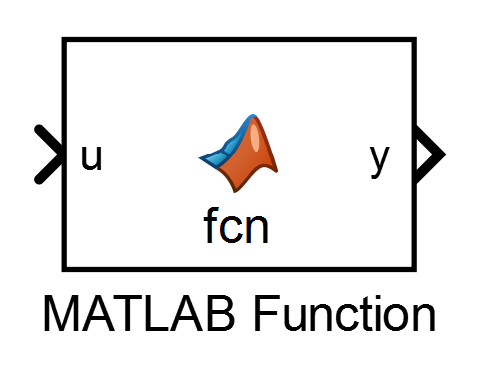
\includegraphics[width=2cm]{matlab_fcn.png}
\caption{Blok MATLAB Function v Simulinku}
\end{figure}
\end{frame}

\begin{frame}[fragile]{Pom�cka}
Zabezpe��me aby Simulink nekompiloval funkciu quadprog, nap�eme funkciu nasledovn�m sp�sobom:
\begin{lstlisting}
function u = fcn(H,G,x,Ac,b0)
%#codegen

u=double(ones(30,1));

% MPC with constrains
coder.extrinsic('optimset','quadprog');
options = optimset('Display','off','Algorithm','active-set');
[u_ast,f]=quadprog(H,G*x,Ac,b0,[],[],[],[],[],options);

u=u_ast;

\end{lstlisting}
\end{frame}

\begin{frame}{Zadanie}
\begin{itemize}
\item Vytvorte simul�ciu riadenia nosn�ka v prostred� simulink
\item Rozbehajte MPC pomocou funckie quadprog
\item Porovnanie simul�cie riadenia Simulink vs. MATLAB v jednom grafe
\item Blokov� sch�mu a MATLAB k�d tie� vlo�te do zadania
\end{itemize}
\end{frame}

\end{document}